\documentclass{beamer}
\usepackage{apacite}
\usepackage{caption}
\usepackage[font=small, labelfont=bf]{subcaption}
\usepackage{textpos}
\usetheme{Darmstadt}
\usepackage{graphicx}
\usepackage{float}
%packages for definitions%%%%%%%%%%%%%%
\usepackage{blindtext}
\usepackage{scrextend}
\addtokomafont{labelinglabel}{\sffamily}
%%%%%%%%%%%%%%%%%%%%%%%%%%%%%%%%%%%%%%%
\AtBeginSection[]{
    \begin{frame}
    \vfill
    \centering
    \begin{beamercolorbox}[sep=8pt,center,shadow=true,rounded=true]{title}
        \usebeamerfont{title}\insertsectionhead\par%
    \end{beamercolorbox}
    \vfill
    \end{frame}
}
\title{Garaphlet Analysis for HiC data}
\author{Behnam Rasoolian}
\institute{Auburn University}
\definecolor{auburn_orange}{RGB}{221, 85, 12}
\definecolor{auburn_blue}{RGB}{3, 36, 77}
\date{}
\begin{document}
\frame{\titlepage}
%\addtobeamertemplate{frametitle}{}{%
%    \begin{textblock*}{100mm}(.8\textwidth,-1.65cm)
%        
\includegraphics[height=1.65cm,width=3cm]{figures/auburn_logo.jpeg}
%    \end{textblock*}}
\section{Biological Background}
\begin{frame}[t]
    \frametitle{Purpose of this research}
    \framesubtitle{Introduction}
    \begin{columns}
        \begin{column}{.5\textwidth}
            \begin{itemize}
                \item In this research we plan to find dissimilarities 
                    between normal cells and cancerous cells.
                \item Ideally, it is desirable to compare \textbf{3D confomation}
                    of genomes in order to make such comparisons.
            \end{itemize}
        \end{column}
        \begin{column}[c]{.5\textwidth}
            \begin{figure}
                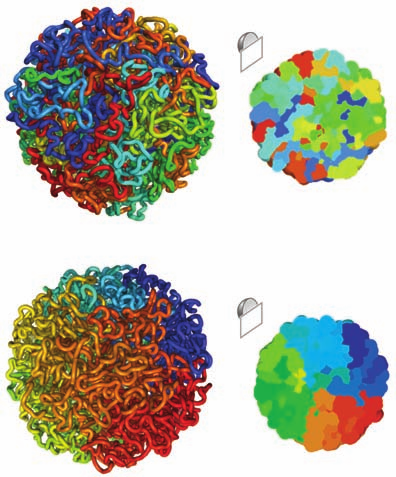
\includegraphics[width=.6\textwidth]{figures/chromosome_3d_structure.png}
                \caption*{ \cite{lieberman2009comprehensive}}
            \end{figure}
        \end{column}
    \end{columns}
\end{frame}

\begin{frame}
    \frametitle{Purpose of this research}
    \framesubtitle{Challenges}
        \begin{columns}
            \begin{column}[c]{.6\textwidth}
                \begin{itemize}
                        \item We still don't have enough information  
                            regarding the exact configuration
                        of a genome inside nucleus.
                        \item However, we can map interactions  in an
                        \textit{HiC contact map} ($C$).
                    \item Rows and columns signify genome fragments.
                    \item $C_{ij} = $ Number/strength of interactions detected between
                        fragment $i$ and $j$.
                \end{itemize}                                                                                 
            \end{column}
            \begin{column}{.4\textwidth}
                \begin{figure}
                    \centering
                    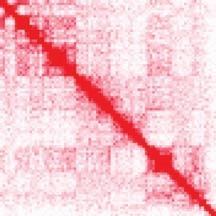
\includegraphics[width=\textwidth]{figures/original_contact_map_chr14.png}
                    \caption*{ \cite{lieberman2009comprehensive}}
                \end{figure}
            \end{column}
        \end{columns}
\end{frame}  
\begin{frame}
    \frametitle{Preliminaries}
    \framesubtitle{What is 3D conformation?}
    If you unfold the DNA inside one of your cells, it would measure
    2 meters end to end. How is it folded up withing a nucleus which
    is only 6 micorns wide?
    \begin{figure}
        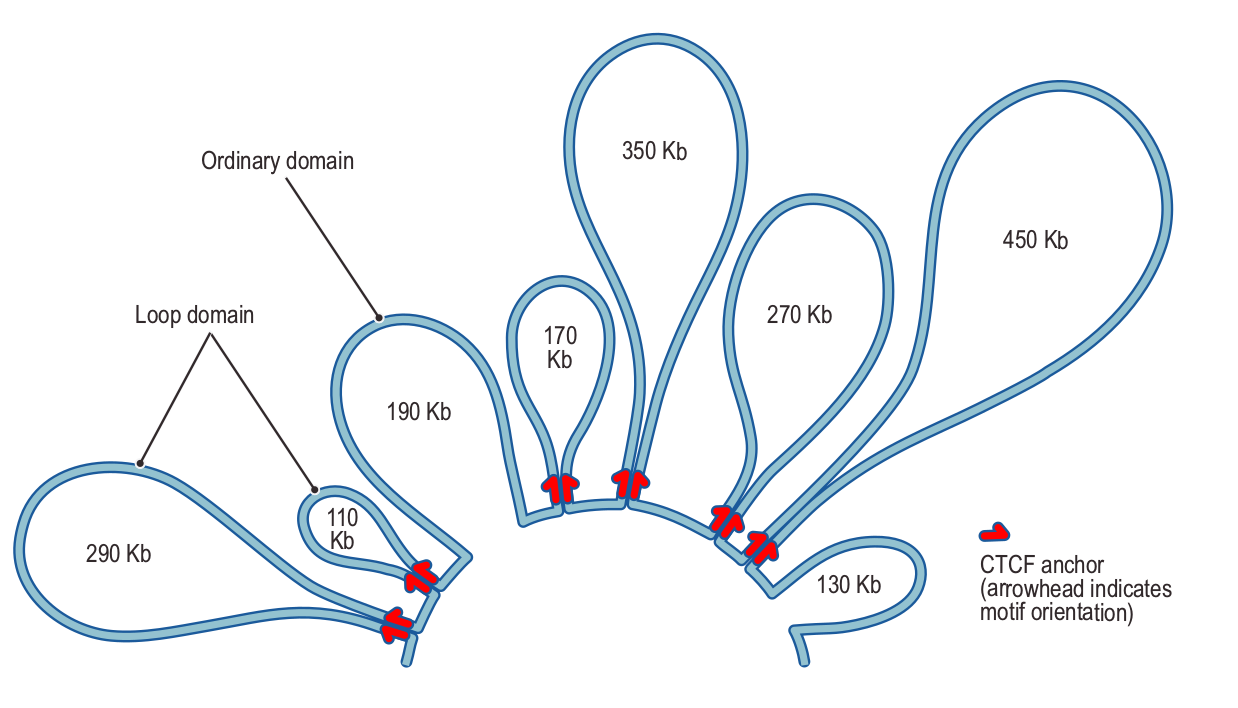
\includegraphics[width=.7\textwidth]{figures/loops.png}
        \caption*{ \cite{rao20143d}}
    \end{figure}
\end{frame}
\begin{frame}
    \frametitle{Preliminaries}
    \framesubtitle{Terminology \cite{wang2013properties}}
    \begin{columns}
        \begin{column}{1.15\textwidth}
     \fontsize{10}{10}\selectfont{
         \begin{itemize}
             \item \textbf{Nucleotide}:  The monomer units that comprise DNAs. There
        are 4 types of nucleotides: (C, G, A, and T)

        \item \textbf{Base}: Each pair of nucleotides in the DNA are called
        a base.
        \\A kilo-base resolution is a resolution that
        corresponds to 1000 pairs of nucleotides in DNA.

        \item \textbf{Nucleosome}: A basic unit 
        consisting of 145-147 bases wrapped around a
        protein complex. 

        \item \textbf{Chromatin Fiber}: Tens of nucleosomes are
        further collapsed into a larger dense structural unit
        of several kilobase (Kb) pairs.

        \item \textbf{Locus}: Multiple chromatin fibers form a large module of megabase pairs 
            (Mb) DNA, which may be referred to as \textit{domains, globules, gene
                 loci, or chromatin clusters} in different contexts.

        \item \textbf{Chromosome}: A number of loci then fold into a large
        independent physical structure, chromosome. 
         \end{itemize} }
        \end{column}
    \end{columns}
\end{frame}
\begin{frame}
    \frametitle{HiC Method}
    \framesubtitle{Procedure}
    \begin{columns}
        \begin{column}{1.1\textwidth}
            \begin{enumerate}
                \item Freeze the DNA in place.
                \item Cut the genome in tiny pieces.
                    Mark the ends using Biotin, and glue them together into
                    diffused pieces of DNA. These diffused pieces is made
                    up of two bits of the genome that are spatial neighbors.
                \item Using DNA sequencing, the two parts of the 
                    diffused DNA are identified and a dataset is created
                    where each cell corresponds to a pair.
            \end{enumerate}
        \end{column}
    \end{columns}
\end{frame}
\begin{frame}
    \frametitle{HiC Method}
    \framesubtitle{Illustration}
    \begin{figure}
        \centering
        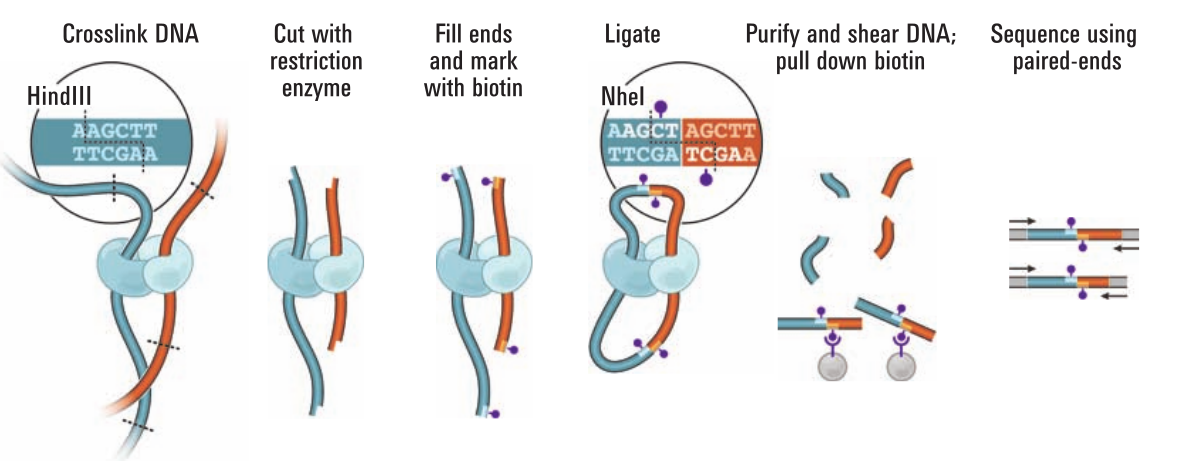
\includegraphics[width=1.1\textwidth]{figures/hic_process.png}
        \caption*{ \cite{lieberman2009comprehensive}}
    \end{figure}
\end{frame}

\begin{frame}
    \frametitle{HiC Method}
    \framesubtitle{Contact Maps}
    \begin{columns}
        \begin{column}{.5\textwidth}
            \begin{itemize}
                \item The whole genome is then divided into sections of certain length (i.e. 500kB or 1MB)
                    and interactions are aggregated over them.
                \item Contact maps can be used to develop both inter- and 
                    intra-chromosomal interaction matrices.

            \end{itemize}
        \end{column}
        \begin{column}{.5\textwidth}
             \begin{figure}[H]
                \centering
                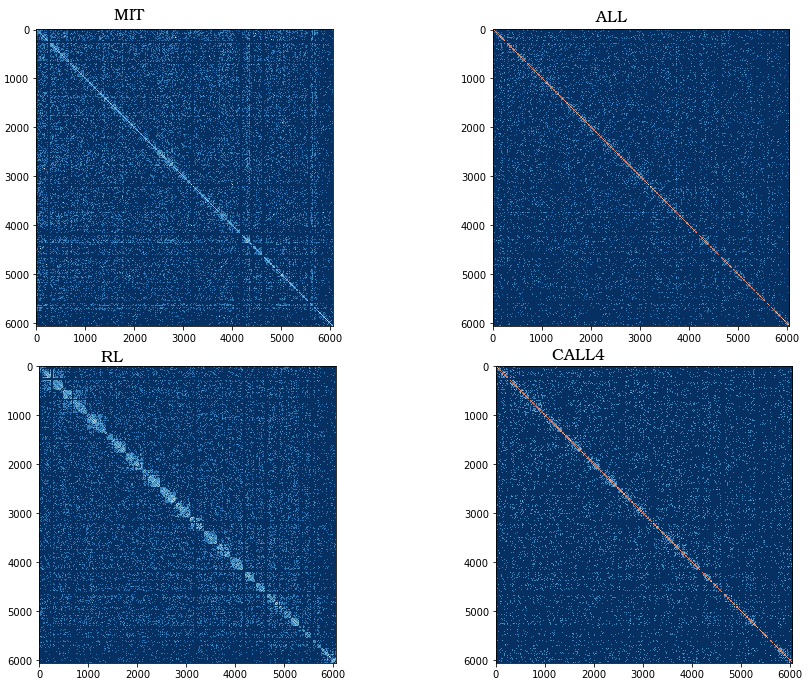
\includegraphics[width=\textwidth]{figures/grand_scheme_of_things.png}
                \caption*{}
            \end{figure}
        \end{column}
    \end{columns}
\end{frame}

\frame{
    \frametitle{HiC Data: An Overal Picture}
     \begin{figure}[H]
        \centering
        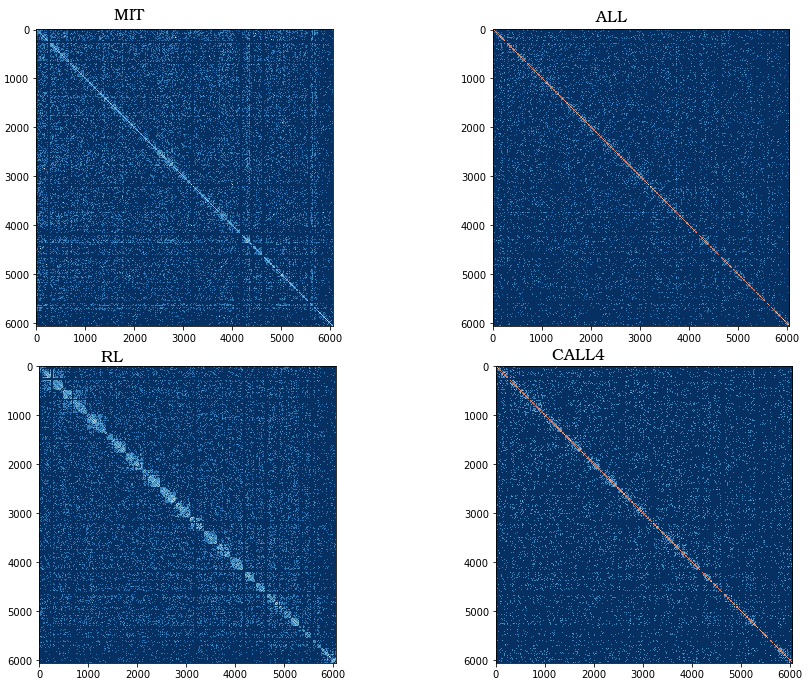
\includegraphics[width=.8\textwidth]{figures/grand_scheme_of_things.png}
        \caption*{}
    \end{figure}

}

\frame {
    \begin{figure}
        \centering
        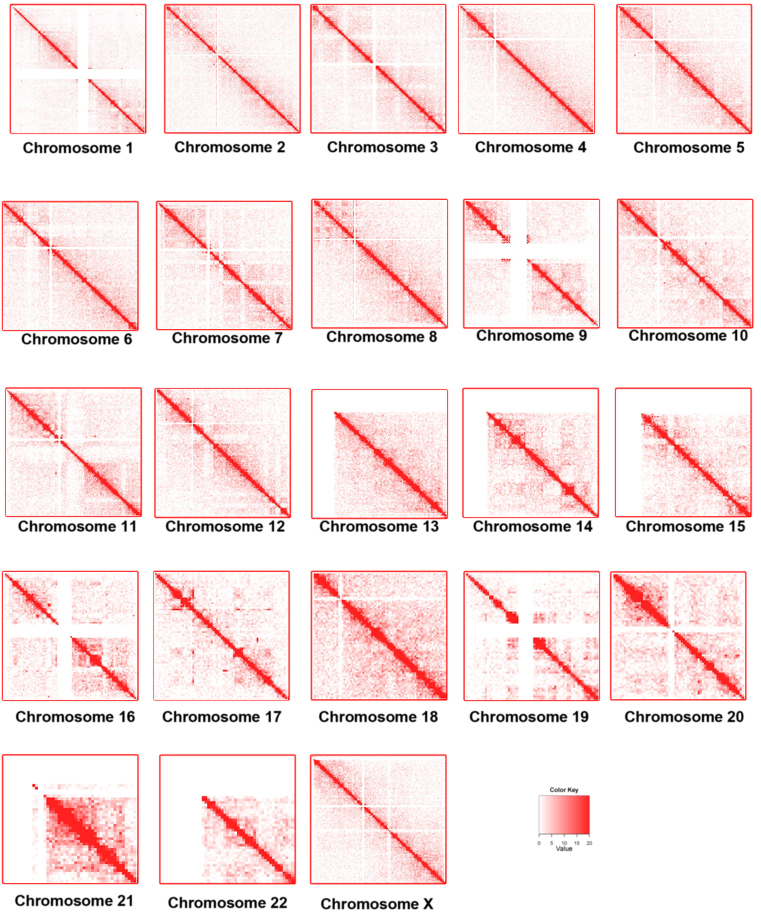
\includegraphics[width=.8\textwidth, height=.82\textheight]{figures/normal-b-cell-all-heatmaps.jpeg}
        \caption*{\cite{wang2013properties}}
    \end{figure}

}

\section{Strategies}
\begin{frame}
    \frametitle{Graphlets}
    \framesubtitle{Definitions}
    Graphlet comparison, introduced by \citeA{prvzulj2007biological},
    is a novel method used to compare large networks in order to
    find local similarities in them.
    \begin{itemize}
        \item \textbf{Fragment:} A connected subgraph.
        \item \textbf{Motifs:} Fragments that occur with a frequency much higher than
            that occuring in a randomly generated graph.
        \item \textbf{Graphlets:} An arbitrary, induced fragment.
        An edge is the only two-node graphlet.
        \item \textbf{Induced graphs:} Given a graph $G(V, E)$ and $S \subseteq V$,
            then $G'(S, E')$
            is a graphlet iff $E' = \{(u, v) | u, v \in V \text{ and } 
            (u, v) \in E \rightarrow (u, v) \in E'\}$
        \item \textbf{Orbits:} Set of all nodes in a graphlet that can be
            swapped with each other while not changing the graph.
    \end{itemize}
\end{frame}

\begin{frame}
    \frametitle{Graphlets}
    \begin{figure}
        \centering
        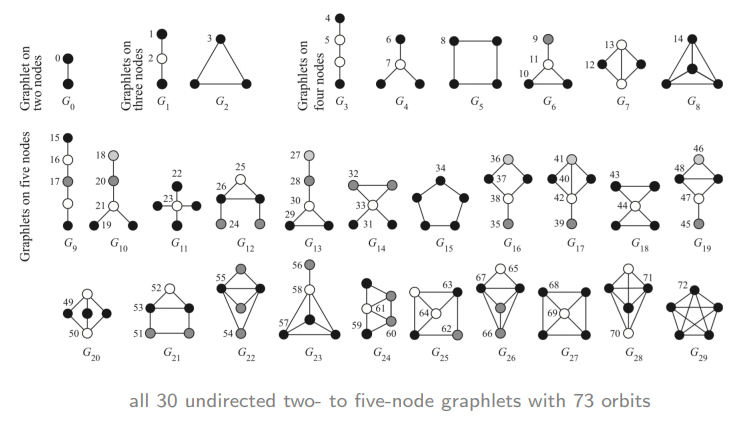
\includegraphics[scale=.4]{graphlets.png}
        \caption*{All 30 undirected two- to five-node
        graphlets with 73 orbits \cite{prvzulj2007biological}}
    \end{figure}
\end{frame}
\begin{frame}
    \frametitle{Graphlets}
    \framesubtitle{Applications}
    \textbf{\citeA{milenkoviae2008uncovering}:}

    \textit{Signature vector:} A 73-dimensional vector
    $\mathbf{s}^T
    = [s_0, s_2, ..., s_{72}]$ where $s_i$ denotes the number of nodes in
    the network that are part of an orbit $i$.
    
    \textit{Important Result}: Proteins with similar surroundings perform
    similar functions.
    \begin{figure}[H]
        \centering
        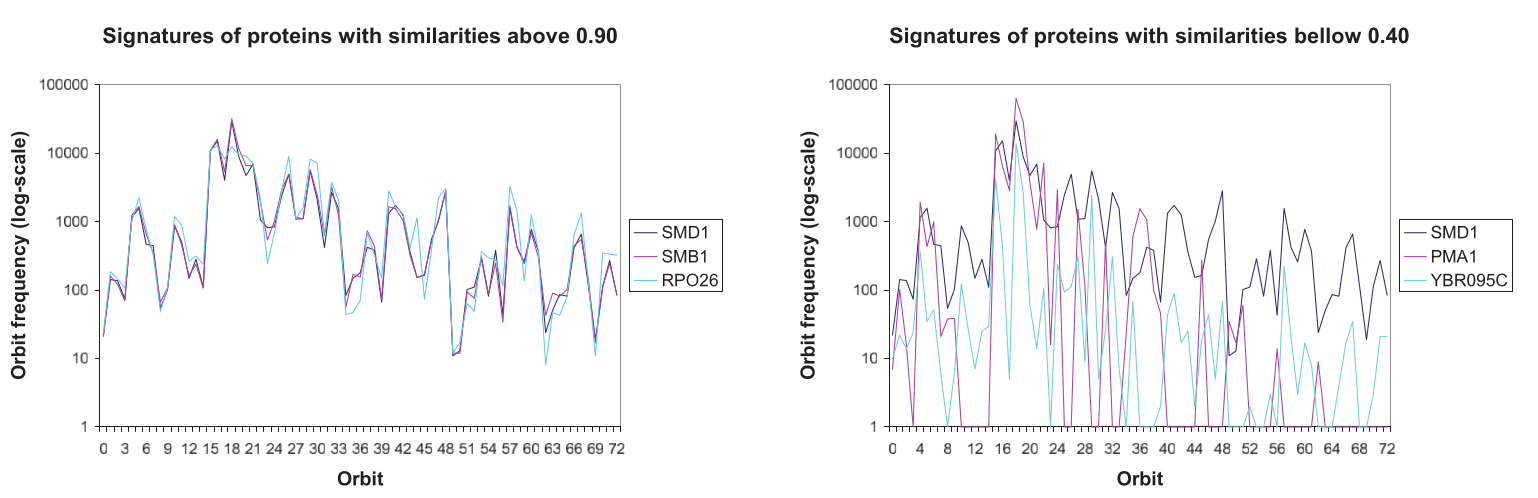
\includegraphics[width=\textwidth]{figures/signature-comparison.png}
        \caption*{\cite{milenkoviae2008uncovering}}
    \end{figure}
\end{frame}

\begin{frame}
    \frametitle{Introduction}
    \textbf{\citeA{milenkovic2010cancer}}: 

    Investigate cancer-causing genes to find similarities in their signatures. 
    \begin{enumerate}
        \item Cluster the genes based on \textit{signature similarity} criteria.
            Some clusters contain a lot of cancerous genes.
        
        \item Predict the cancer-relatedness of a protein $i$ using
            an enrichment criteria $\frac{k}{|C_i|}$ \\
            \begin{itemize}
                \item $C_i$ : the cluster where protein $i$ belongs\\
                \item $k$ : the number of cancer-causing proteins in $C_i$ \\
                \item $|C_i|$ : the size of $C_i$
            \end{itemize}
    \end{enumerate}
\end{frame}

\frame {
    \frametitle{Stage I: Thresholding}
    For thresholding, I use \textit{local thresholding} methods.
    \begin{enumerate}
        \item Create a zero matrix with the same size as the contact 
            map (M)
        \item Slide a kernel through each pixel
        \item If the pixel $(i, j)$  satisfies a particular condition
            the set $A[i, j]$.
    \end{enumerate}
    \bigskip
    Conditions that I considered:
    \begin{enumerate}
        \item If the pixel is local maximum with respect to the pixels
            that fall in the kernel \\
            $A_{ij} > A_{i',j'} 
            \hspace{2cm}  (i', j') \in \{i-k, i+k\}\times \{j-k, j+k\}$
        \item If the pixel value is larger that some standard deviation
            from the mean of the values that fall inside the kernel.
            $A_{ij} > mean(A_{i',j'}) + std(A_{i',j'})$ \\
    \end{enumerate}
}

\frame {
    \frametitle{Kernels}
    \begin{figure}[H]
        \centering
        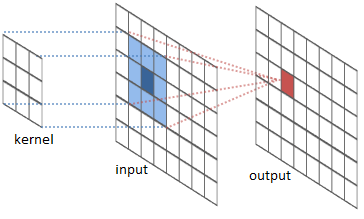
\includegraphics[width=.9\textwidth]{figures/kernels.png}
        \caption*{}
    \end{figure}
}

\frame {
    \frametitle{Thresholding example}
    \begin{figure}[H]
        \centering
        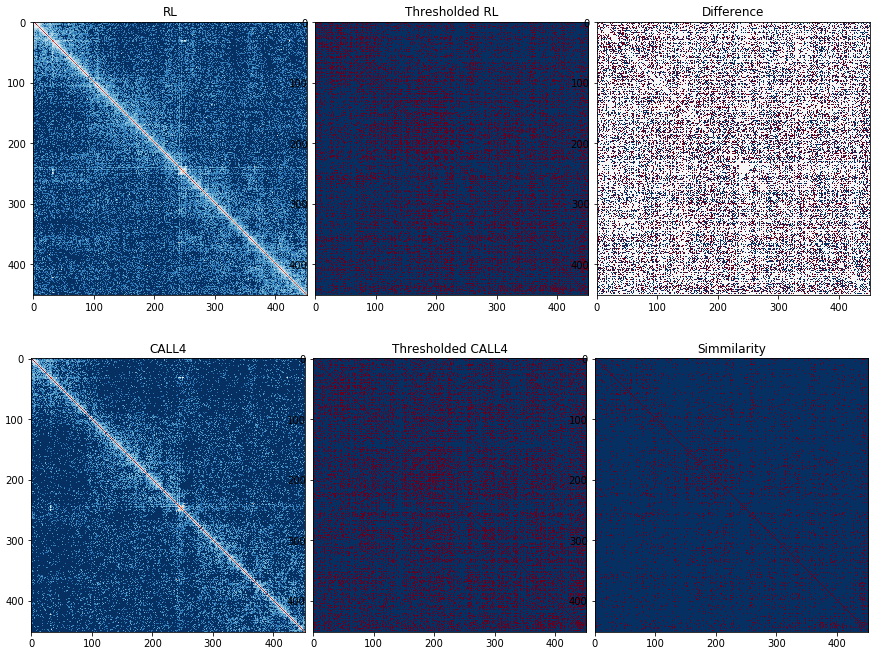
\includegraphics[height=.8\textheight]{figures/thresholding_example.png}
        \caption*{}
    \end{figure}
}

\frame {
    \frametitle { Extracting graphlets }
    \begin{enumerate}
        \item I used the \texttt{orca} library in \texttt{R} programming 
        language.
        \item For each loci, a \textit{signature vector} of length 73 is 
        created.
        \item For each chromosome, an $N_c \times 73$, matrix is returned.
        where $N_c$ is the number of loci in chromosome $c$.
    \end{enumerate}
}

\frame {
    \frametitle { Extracting graphlets }
    \begin{figure}[H]
        \centering
        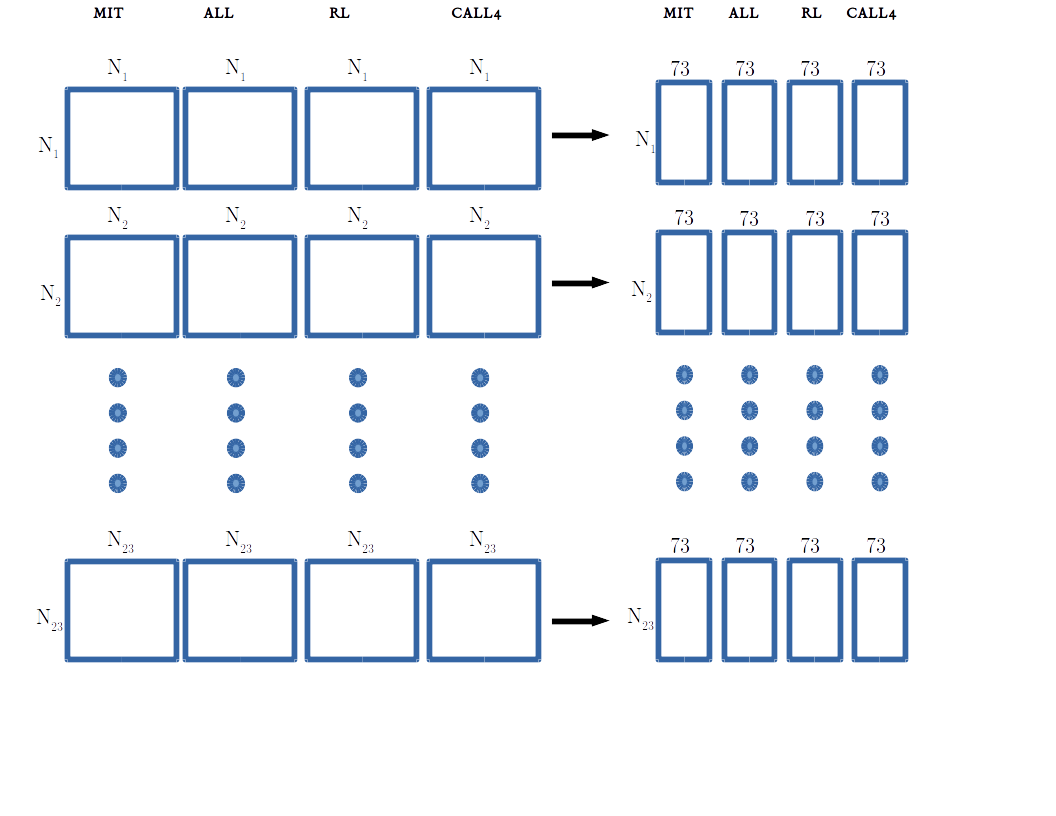
\includegraphics[width=.9\textwidth]{figures/graphlet_extraction.png}
        \caption*{}
    \end{figure}
}
\frame {
    \frametitle { Finding distance between loci }
    In order to see how different two loci are in 
    terms of local neighborhood, we need to compare
    their corresponding \textit{signature values}.
    The distance measure proposed by \citeA{prvzulj2007biological}:

    \begin{equation}
        d_i = w_i \times \frac{log(S_i+1) - log(S'_i+1)}{log(max(S_i, S'_i) + 2)}
    \end{equation}
    The distance between $S$ and $S'$ can be calculated as follows:
    \begin{equation}
        D = \sum_{0}^{72}{d_i^2}
    \end{equation}
}

\section{Loci Signature Comparison Among Cells}

\frame {
    \frametitle{Loci-loci distances between cell lines}
    I calculated loci-loci distance between cell lines using the formula
    above:
    \begin{figure}[H]
        \centering
        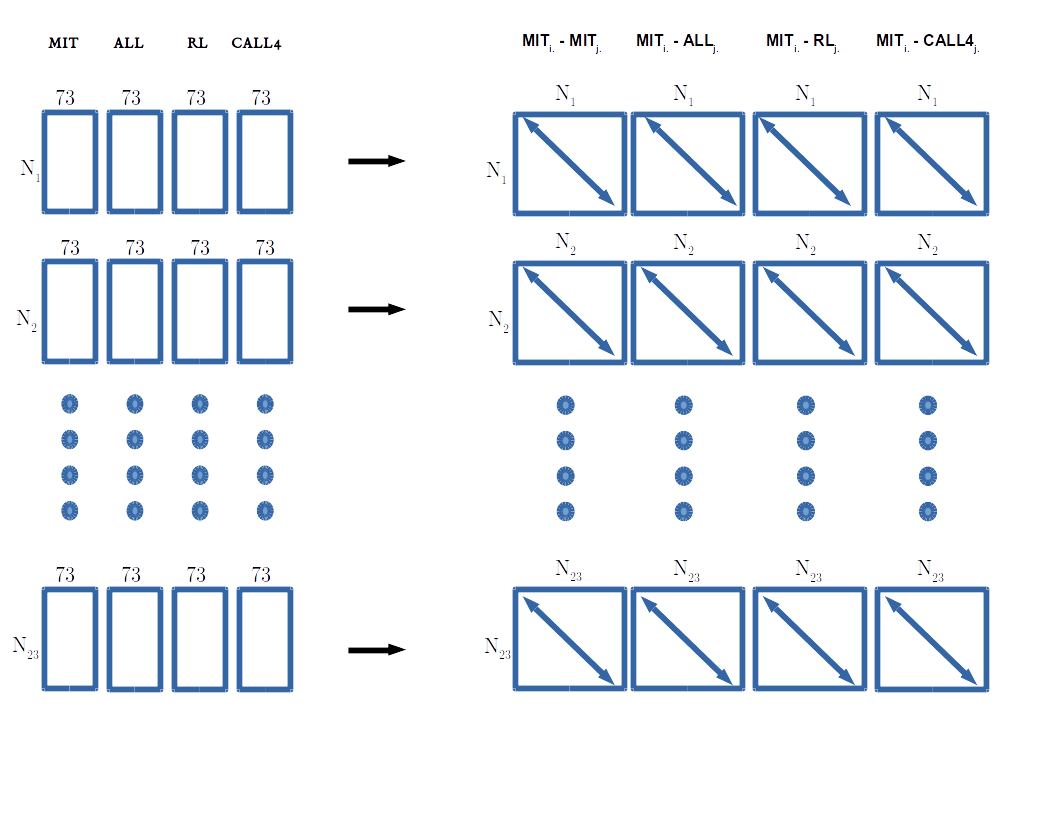
\includegraphics[width=.85\textwidth]{figures/graphlet_distance_extraction.png}
        \caption*{}
    \end{figure}
}
\frame{
    \frametitle{Loci-loci distance between cell lines}
    \begin{figure}[H]
        \centering
        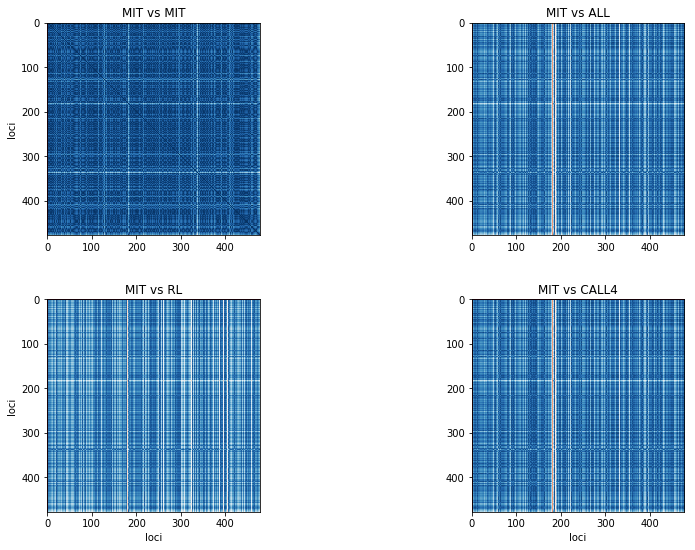
\includegraphics[width=.6\textwidth]{figures/loci_wise_distance.png}
        \caption*{\small {$A_{ij}$ in matrices above denotes distance between loci
        $i$ in row cell line and loci $j$ in the column cell line.} }
    \end{figure}
}
\frame {
    \frametitle{Loci-loci distances}
    \begin{figure}[H]
        \centering
        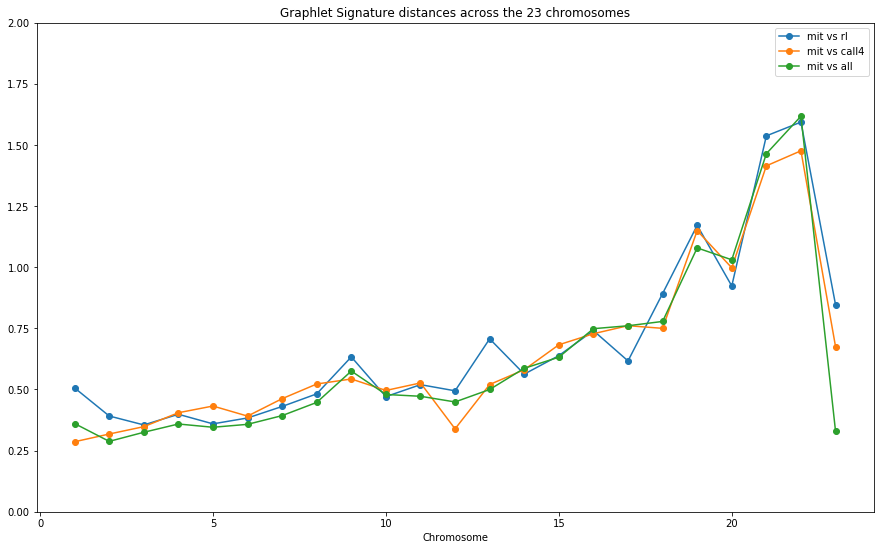
\includegraphics[width=\textwidth]{figures/cross_chromosomal_signature_distance.png}
        \caption*{}
    \end{figure}
}

\frame {
    \frametitle{Loci-loci distances}
    \begin{figure}[H]
        \centering
        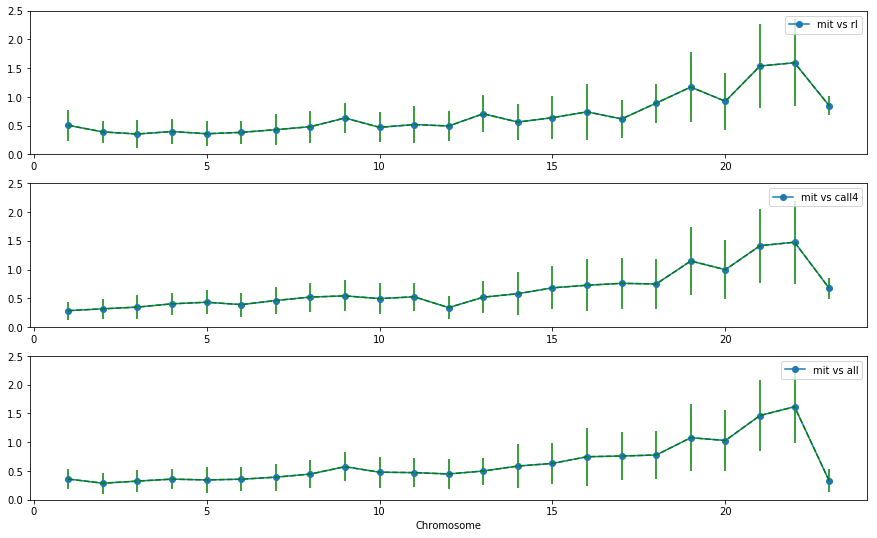
\includegraphics[width=\textwidth]{figures/cross_chromosomal_signature_distance_separated.png}
        \caption*{cross-chromosomal signature distance with 1 standard deviation error bars}
    \end{figure}
}

\section{Orbit Distribution correlation Comparison Among Cells}

\frame {
    \frametitle{Orbit correlations}
    \begin{figure}[H]
        \centering
        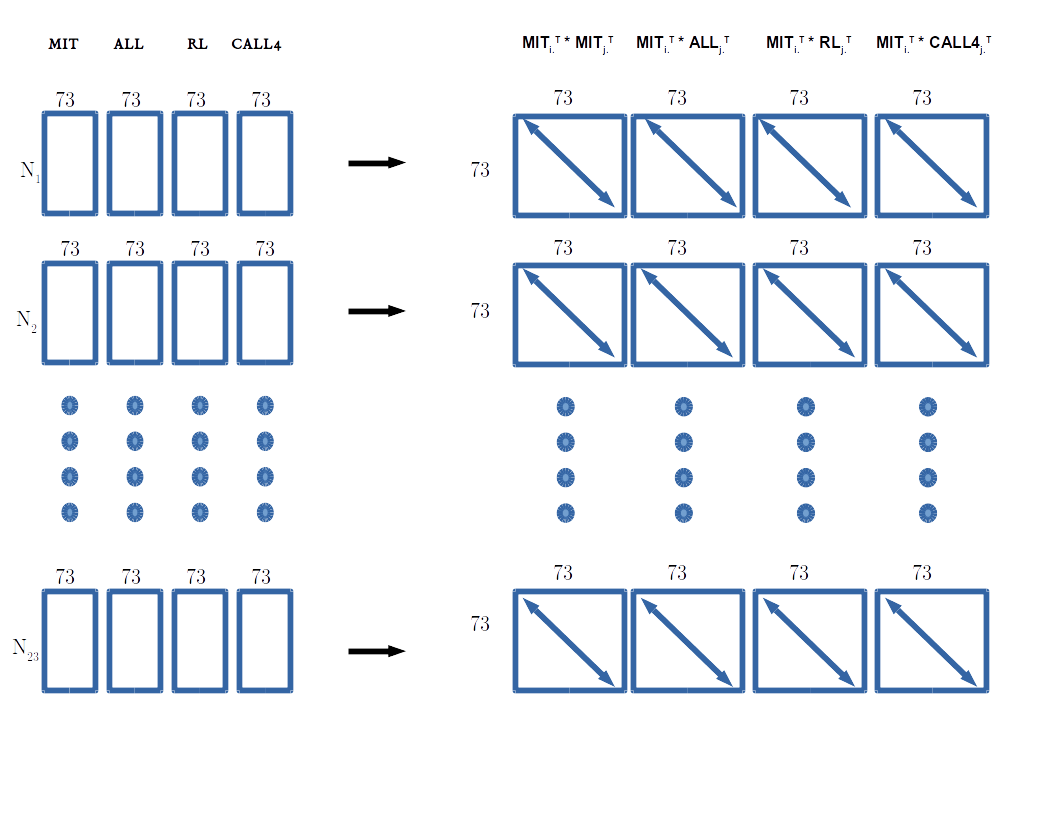
\includegraphics[width=\textwidth]{figures/orbit_distribution_comparison.png}
        \caption*{}
    \end{figure}
}

\begin{frame}
    \frametitle{Orbit distribution comparison among cells}
    \begin{figure}[H]
        \centering
        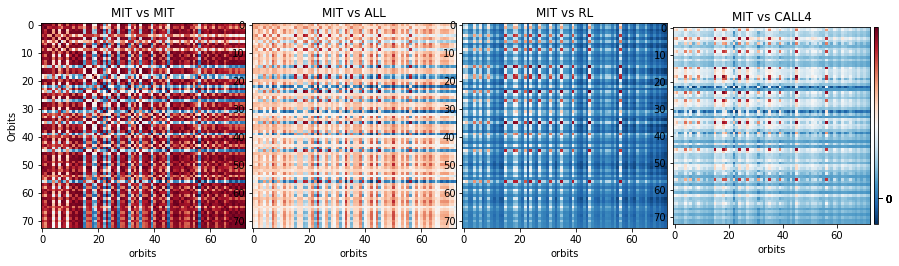
\includegraphics[width=\textwidth]{figures/orbit_wise_correlation_chr1.png}
        \caption*{\small {$A_{ij}$ in matrices above denotes correlation between 
        orbit $i$ in row cell line and orbit $j$ in the column cell line.} }
    \end{figure}
\end{frame}

\frame {
    \begin{figure}[H]
        \centering
        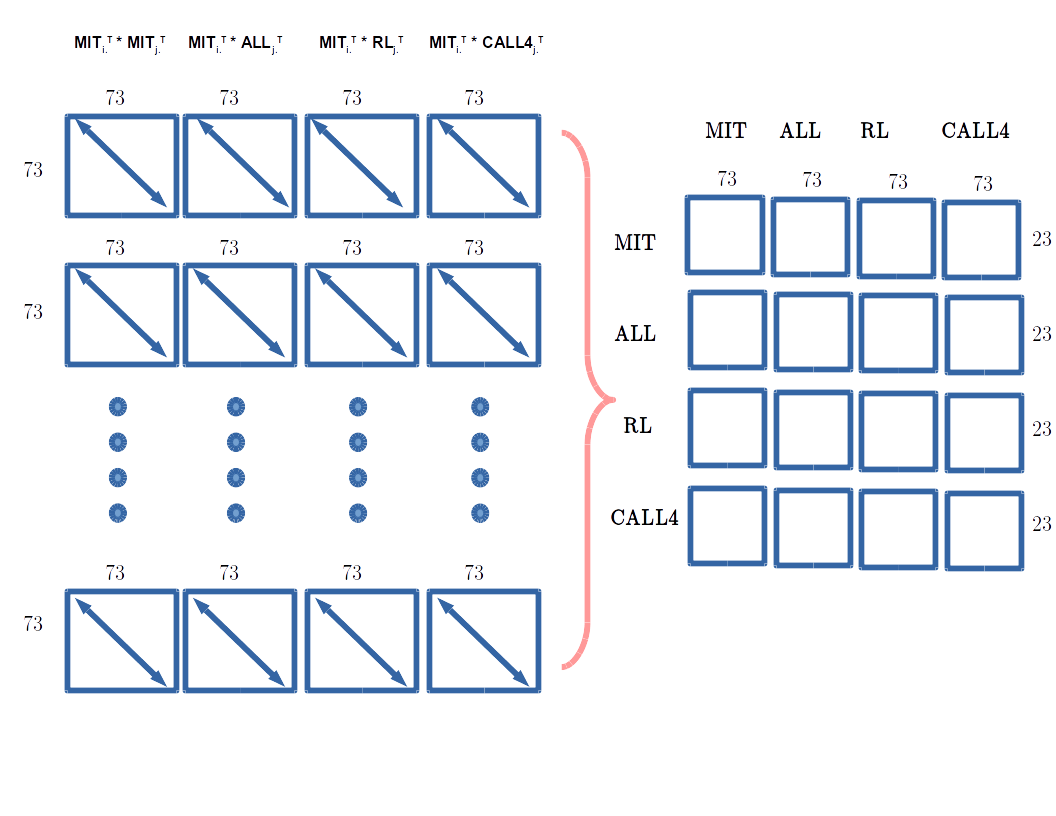
\includegraphics[width=\textwidth]{figures/graphlet_correlation_aggregation.png}
        \caption*{}
    \end{figure}
}
\frame {
    \frametitle{Comparison of mean correlation among all orbits across the 23 chromosomes.}
    \begin{figure}[H]
        \centering
        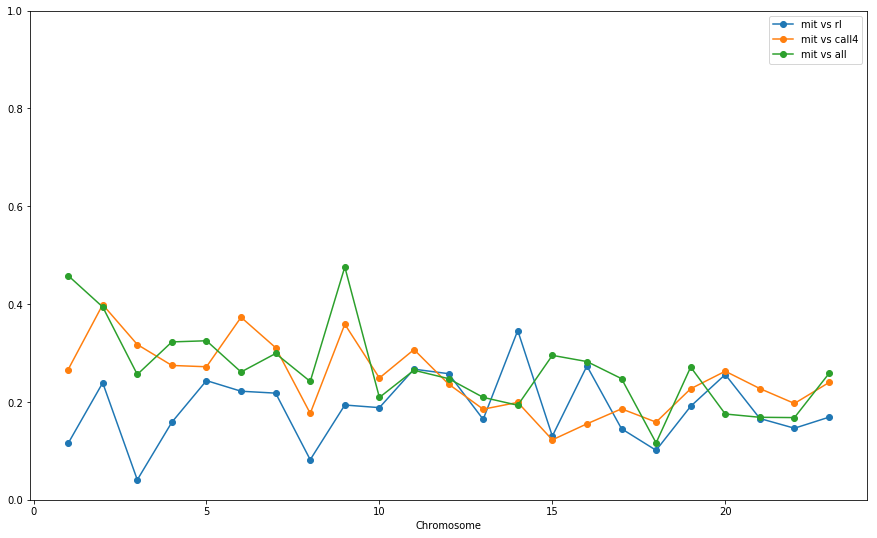
\includegraphics[width=\textwidth]{figures/graphlet_correlation_comparison_chromosomes.png}
    \end{figure}
}

\frame {
    \frametitle{Comparison of mean correlation among all orbits across the 23 chromosomes.}
    \begin{figure}[H]
        \centering
        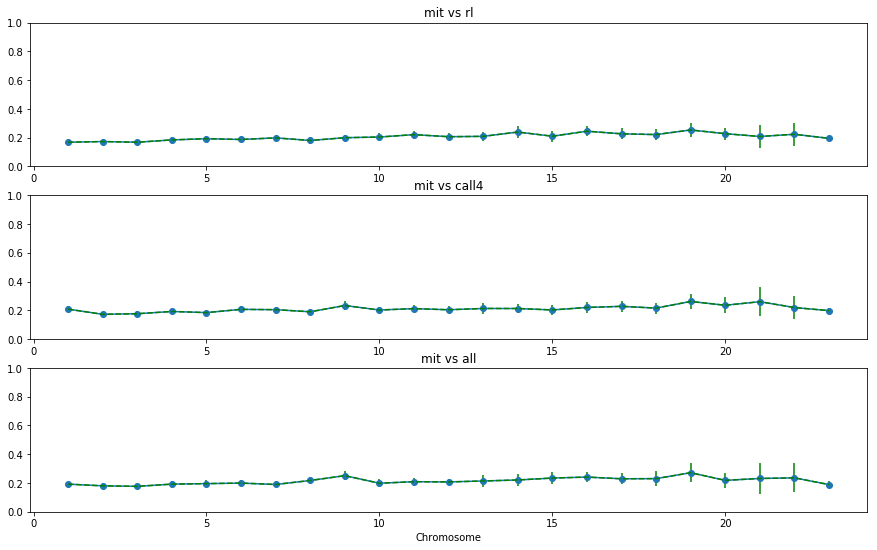
\includegraphics[width=\textwidth]{figures/graphlet_correlation_comparison_chromosomes_separated.png}
    \end{figure}
}

\frame {
    \frametitle{Comparison of mean correlation among all chromosomes across the 73 orbits.}
    \begin{figure}[H]
        \centering
        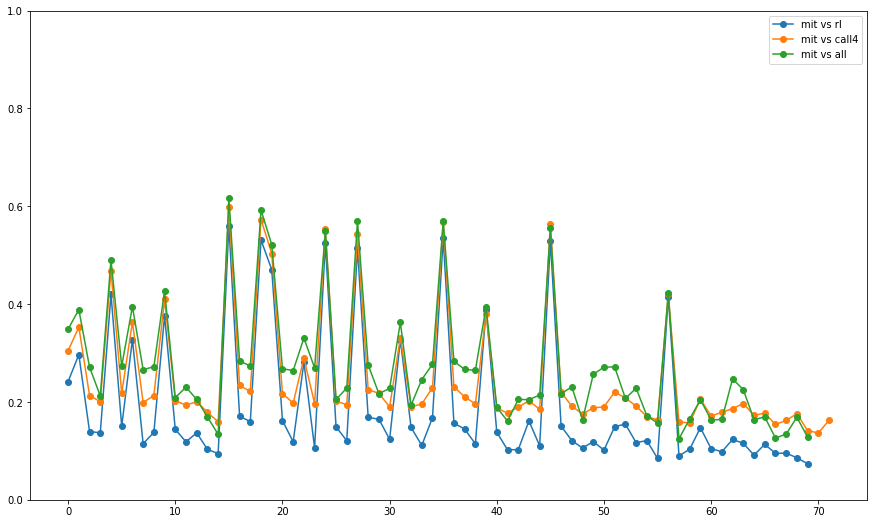
\includegraphics[width=\textwidth]{figures/graphlet_correlation_comparison_orbits.png}
    \end{figure}
}

\frame {
    \frametitle{Comparison of mean correlation among all chromosomes across the 73 orbits.}
    \begin{figure}[H]
        \centering
        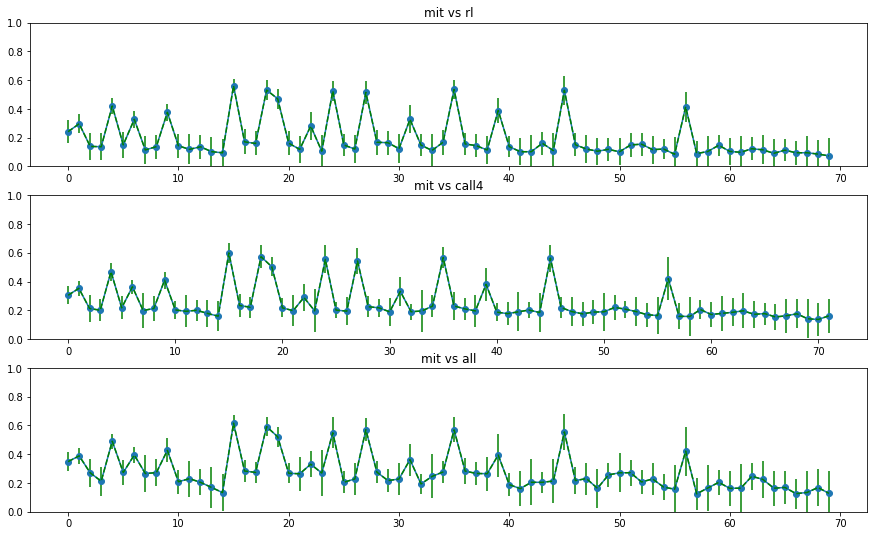
\includegraphics[width=\textwidth]{figures/graphlet_correlation_comparison_orbits_separate.png}
    \end{figure}
}

\section{Orbit Distribution MIC Comparison Among Cells}
\frame {
    \frametitle{About MIC}
    A powerfull method that captures both functional and 
    non-functional relationships.

    \begin{equation}
        MIC(X, Y) = \mathbb{KL}(p(X, Y), p(X)p(Y)
    \end{equation}
}
\frame {
    \frametitle{Comparison of mean MIC among all chromosomes across the 23 chromosomes.}
    \begin{figure}[H]
        \centering
        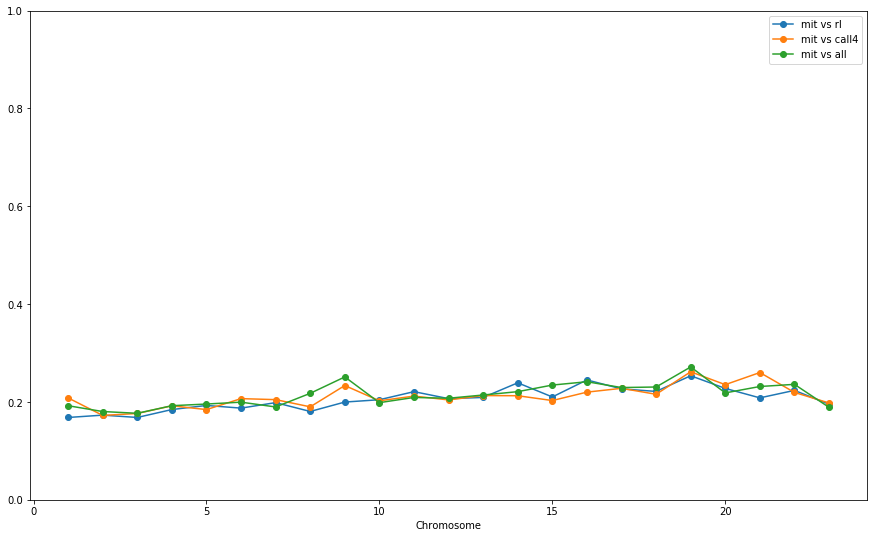
\includegraphics[width=\textwidth]{figures/graphlet_mic_comparison_chromosomes.png}
    \end{figure}
}

\frame {
    \frametitle{Comparison of mean MIC among all chromosomes across the 23 chromosomes.}
    \begin{figure}[H]
        \centering
        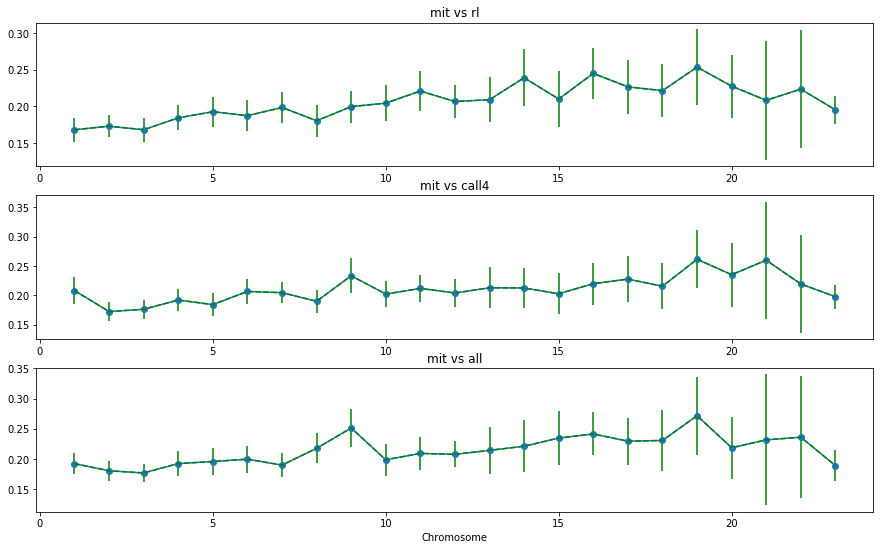
\includegraphics[width=\textwidth]{figures/graphlet_mic_comparison_chromosomes_separate.png}
    \end{figure}
}

\frame {
    \frametitle{Comparison of mean MIC among all chromosomes across the 73 orbits.}
    \begin{figure}[H]
        \centering
        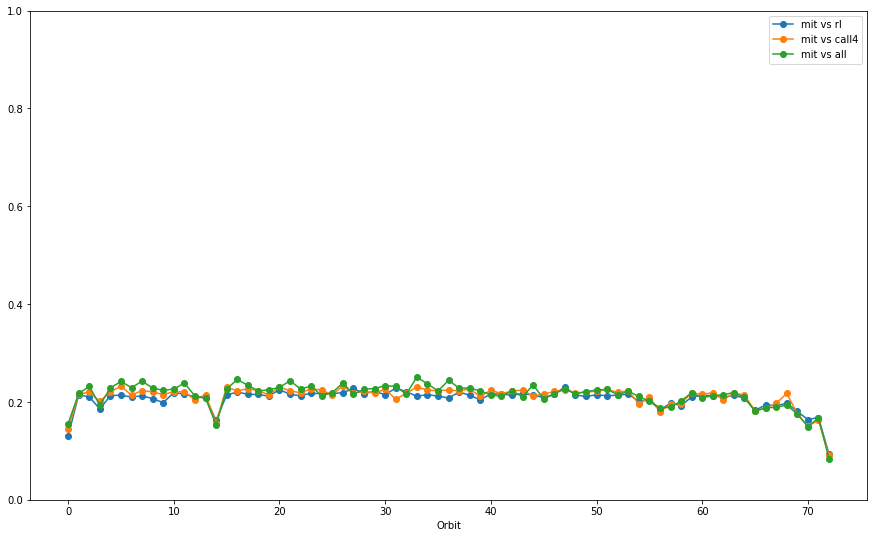
\includegraphics[width=\textwidth]{figures/graphlet_mic_comparison_orbits.png}
    \end{figure}
}

\frame {
    \frametitle{Comparison of mean MIC among all chromosomes across the 73 orbits.}
    \begin{figure}[H]
        \centering
        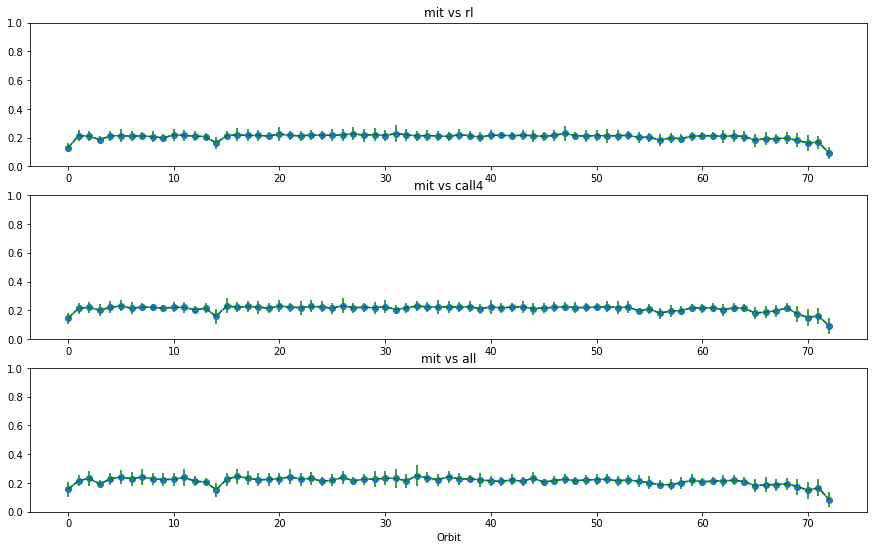
\includegraphics[width=\textwidth]{figures/graphlet_mic_comparison_orbits_separate.png}
    \end{figure}
}



\section{Correlation and MIC comparison}

\frame {
    \frametitle{Comparison of mean MIC among all chromosomes across the 73 orbits.}
    \begin{figure}[H]
        \centering
        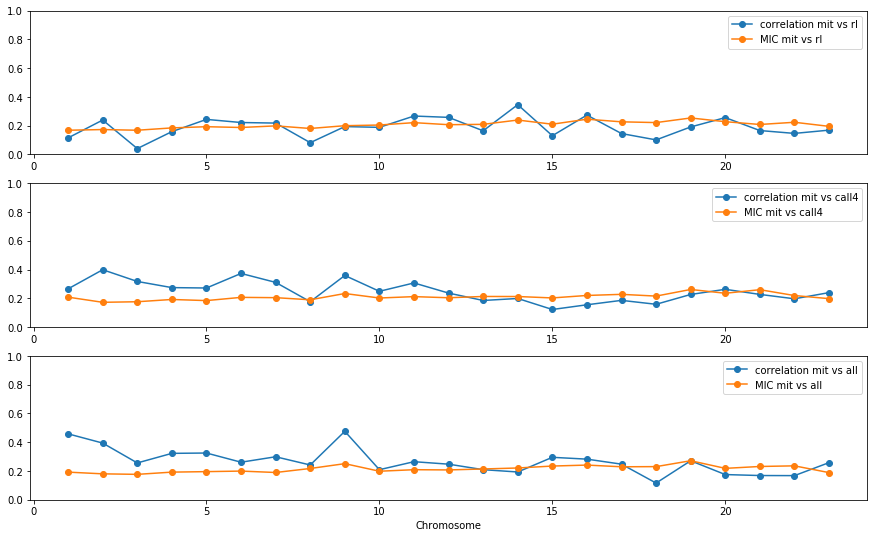
\includegraphics[width=\textwidth]{figures/graphlet_correlation_mic_comparison_chromosomes.png}
    \end{figure}
}


\frame {
    \frametitle{Comparison of mean MIC among all chromosomes across the 73 orbits.}
    \begin{figure}[H]
        \centering
        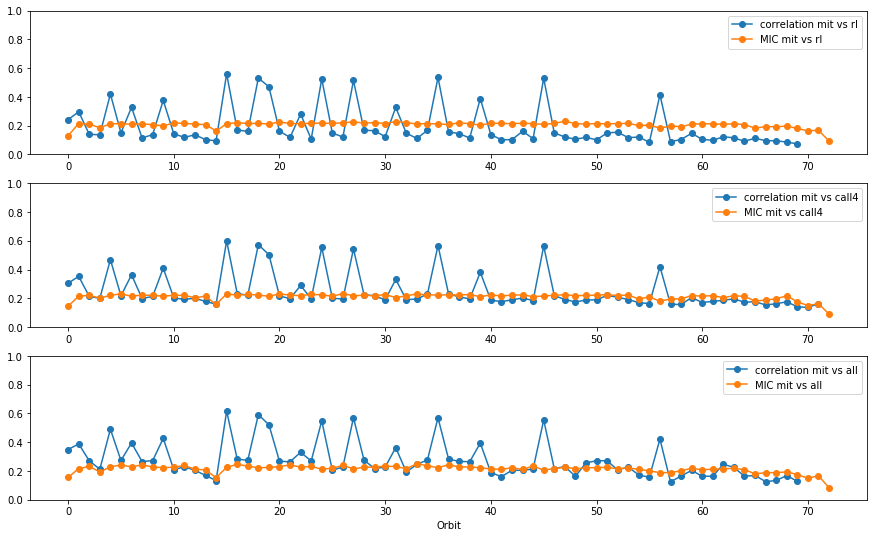
\includegraphics[width=\textwidth]{figures/graphlet_correlation_mic_comparison_orbits.png}
    \end{figure}
}
\section{Cancer Cell Comparison}
\frame {
    \frametitle{Cancer cell MIC comparison}
    \begin{figure}[H]
        \centering
        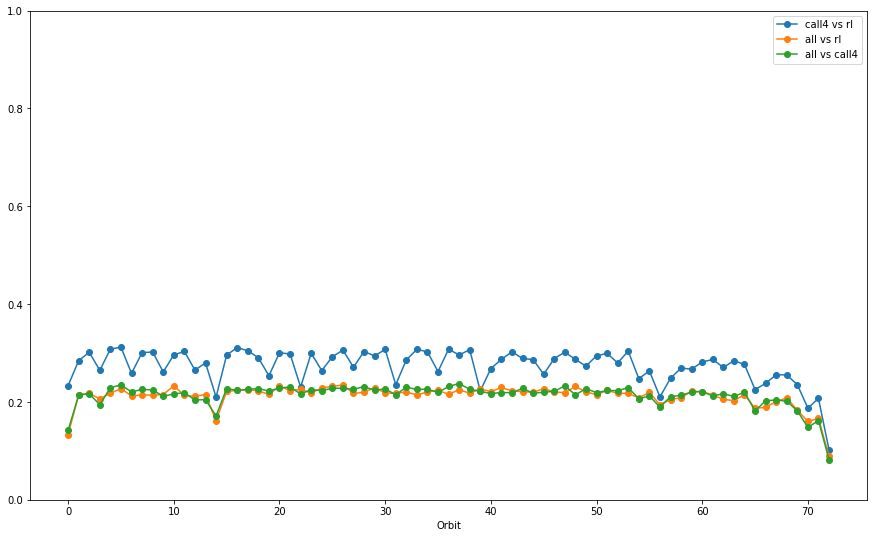
\includegraphics[width=\textwidth]{figures/graphlet_mic_comparison_orbits_cancer.png}
        \caption*{}
    \end{figure}
}

\frame {
    \frametitle{Cancer cell correlation comparison}
    \begin{figure}[H]
        \centering
        \begin{subfigure}[b]{\textwidth}
            \centering
            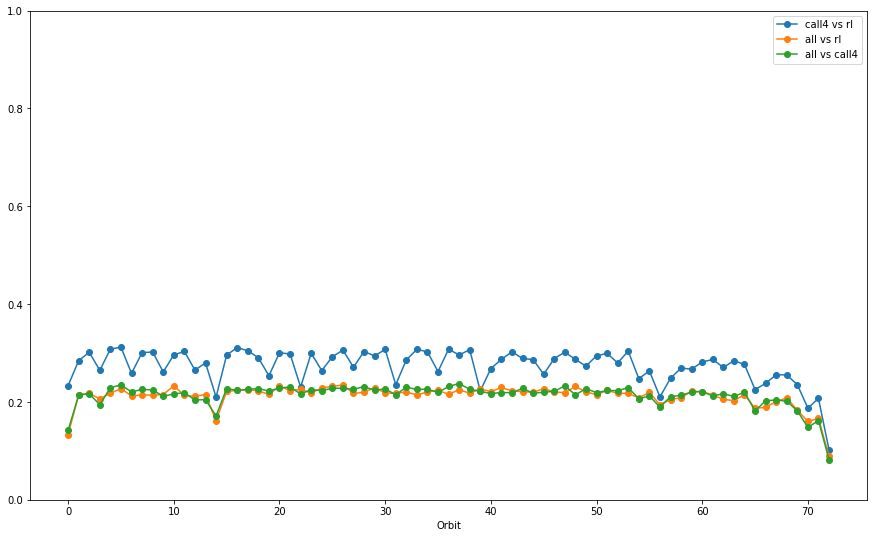
\includegraphics[width=.8\textwidth, height=.35\paperheight]{figures/graphlet_mic_comparison_orbits_cancer.png}
        \end{subfigure}
        \begin{subfigure}[b]{\textwidth}
            \centering
            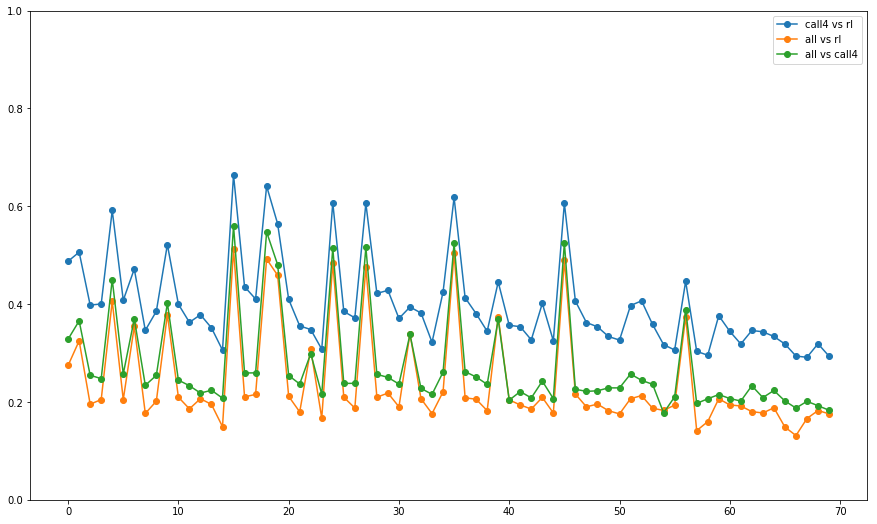
\includegraphics[width=.8\textwidth, height=.35\paperheight]{figures/graphlet_correlation_comparison_orbits_cancer.png}
        \end{subfigure}
        \caption*{}
    \end{figure}
}

\frame {
    \frametitle{Cancer cell correlation comparison}
    \begin{figure}[H]
        \centering
        \begin{subfigure}[b]{\textwidth}
            \centering
            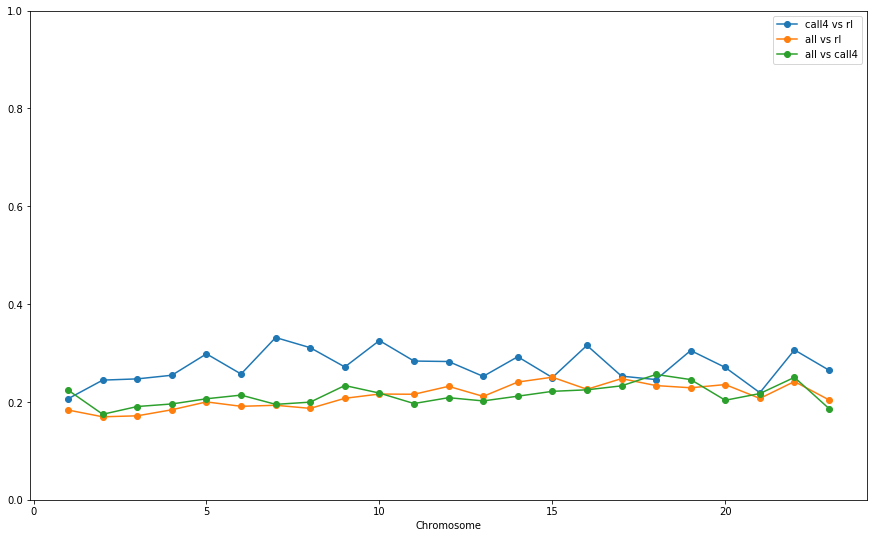
\includegraphics[width=.8\textwidth, height=.35\paperheight]{figures/graphlet_mic_comparison_chromosomes_cancer.png}
        \end{subfigure}
        \begin{subfigure}[b]{\textwidth}
            \centering
            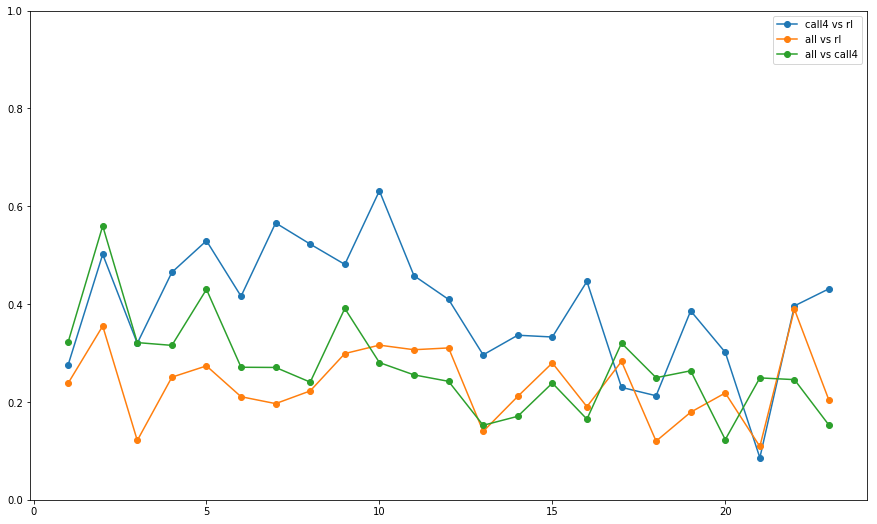
\includegraphics[width=.8\textwidth, height=.35\paperheight]{figures/graphlet_correlation_comparison_chromosomes_cancer.png}
        \end{subfigure}
        \caption*{}
    \end{figure}
}

\begin{frame}[allowframebreaks]
    \frametitle{References}
    \bibliographystyle{apacite}
    \bibliography{lit}
\end{frame}

\end{document}
